%==============================================================================
% Sjabloon onderzoeksvoorstel bachproef
%==============================================================================
% Gebaseerd op document class `hogent-article'
% zie <https://github.com/HoGentTIN/latex-hogent-article>

% Voor een voorstel in het Engels: voeg de documentclass-optie [english] toe.
% Let op: kan enkel na toestemming van de bachelorproefcoördinator!
\documentclass{hogent-article}

% Invoegen bibliografiebestand
\addbibresource{voorstel.bib}

% Informatie over de opleiding, het vak en soort opdracht
\studyprogramme{Professionele bachelor toegepaste informatica}
\course{Bachelorproef}
\assignmenttype{Onderzoeksvoorstel}
% Voor een voorstel in het Engels, haal de volgende 3 regels uit commentaar
% \studyprogramme{Bachelor of applied information technology}
% \course{Bachelor thesis}
% \assignmenttype{Research proposal}

\usepackage{fixltx2e}
\usepackage{comment}

\academicyear{2023-2024}

\title{De toepasbaarheid van goedkope sensoren om gassen in stalomgeving te meten}

%Meten van gassen in ruimten en stallen

%Hoe geschikt zijn goedkope sensoren om gassen in stalomgevingen te meten?

%de werking achter breakoutboards die gasconcentraties kunnen meten en onderzoek naar hoe geschikt ze zijn om gassen in stalomgevingen te meten


\author{Kamiel Halsberghe}
\email{kamiel.halsberghe@student.hogent.be}



\supervisor[Co-promotor]{Pieter-Jan De Temmerman (ILVO Vlaanderen, \href{pieter-jan.detemmerman@ilvo.vlaanderen.be}{pieter-jan.detemmerman@ilvo.vlaanderen.be})}

% Binnen welke specialisatierichting uit 3TI situeert dit onderzoek zich?
% Kies uit deze lijst:
%
% - Mobile \& Enterprise development
% - AI \& Data Engineering
% - Functional \& Business Analysis
% - System \& Network Administrator
% - Mainframe Expert
% - Als het onderzoek niet past binnen een van deze domeinen specifieer je deze
%   zelf
%
\specialisation{Mobile \& Enterprise development}
\keywords{Internet of Things, MQ Sensor, Arduino}

\begin{document}


\begin{abstract}
  
  %Hier schrijf je de samenvatting van je voorstel, als een doorlopende tekst van één paragraaf. Let op: dit is geen inleiding, maar een samenvattende tekst van heel je voorstel met inleiding (voorstelling, kaderen thema), probleemstelling en centrale onderzoeksvraag, onderzoeksdoelstelling (wat zie je als het concrete resultaat van je bachelorproef?), voorgestelde methodologie, verwachte resultaten en meerwaarde van dit onderzoek (wat heeft de doelgroep aan het resultaat?).
  
  
  %Dit onderzoek richt zich op het ontwikkelen en evalueren van goedkope gassensoren, met name MQ-sensoren, die via breakout boards de luchtkwaliteit in varkensstallen kunnen meten. De motivatie voor dit onderzoek ligt in de problematiek van schadelijke stalgassen die een bedreiging vormen voor zowel dieren als mensen, alsook voor de biodiversiteit in de omgeving van de stal. Omdat professionele gassensoren zeer duur zijn en niet thuishoren in een stalomgeving, zou deze studie als inspiratie kunnen dienen voor onderzoekers en fabrikanten van gassensoren, om nieuwe producten te maken die geschikt zijn om in een stalomgeving te werken. De methodologie omvat een literatuurstudie, de bouw en programmering van de sensor en databank, experimenten zowel binnen- als buitenshuis, een vergelijkende test met een professionele gassensor, en een analyse van de verzamelde gegevens. Uit dit onderzoek zou een breakoutboard met meerdere gassensoren komen die in staat is de luchtkwaliteit van een stal te bepalen.
  
  Dit onderzoek richt zich op het ontwikkelen en evalueren van goedkope gassensoren, met name MQ-sensoren, die via breakout boards de luchtkwaliteit in varkensstallen kunnen meten. De motivatie voor dit onderzoek ligt in de problematiek van schadelijke stalgassen die een bedreiging vormen voor zowel dieren als mensen, alsook voor de biodiversiteit in de omgeving van de stal. Omdat professionele gassensoren zeer duur zijn en niet thuishoren in een stalomgeving, zou deze studie als inspiratie kunnen dienen voor onderzoekers en fabrikanten van gassensoren, om nieuwe producten te maken die geschikt zijn om in een stalomgeving te werken. De methodologie omvat een literatuurstudie, de bouw en programmering van de sensor en databank, experimenten zowel binnen- als buitenshuis, en een analyse van de verzamelde gegevens. Uit dit onderzoek zou een breakoutboard met meerdere gassensoren komen die in staat is de luchtkwaliteit van een stal te bepalen.
  

\end{abstract}

\tableofcontents

% De hoofdtekst van het voorstel zit in een apart bestand, zodat het makkelijk
% kan opgenomen worden in de bijlagen van de bachelorproef zelf.
%---------- Inleiding ---------------------------------------------------------


%TODO
% -kost NodeMCU geld?
% -thingsboard API
% -mail sturen pieterjan
% -mail promotor


\section{Introductie}%
\label{sec:introductie}

\begin{comment}

Waarover zal je bachelorproef gaan? Introduceer het thema en zorg dat volgende zaken zeker duidelijk aanwezig zijn:

\begin{itemize}
  \item kaderen thema
  \item de doelgroep -> varkenshouders
  \item de probleemstelling en (centrale) onderzoeksvraag
  \item de onderzoeksdoelstelling
\end{itemize}

Denk er aan: een typische bachelorproef is \textit{toegepast onderzoek}, wat betekent dat je start vanuit een concrete probleemsituatie in bedrijfscontext, een \textbf{casus}. Het is belangrijk om je onderwerp goed af te bakenen: je gaat voor die \textit{ene specifieke probleemsituatie} op zoek naar een goede oplossing, op basis van de huidige kennis in het vakgebied.

De doelgroep moet ook concreet en duidelijk zijn, dus geen algemene of vaag gedefinieerde groepen zoals \emph{bedrijven}, \emph{developers}, \emph{Vlamingen}, enz. Je richt je in elk geval op it-professionals, een bachelorproef is geen populariserende tekst. Eén specifiek bedrijf (die te maken hebben met een concrete probleemsituatie) is dus beter dan \emph{bedrijven} in het algemeen.

Formuleer duidelijk de onderzoeksvraag! De begeleiders lezen nog steeds te veel voorstellen waarin we geen onderzoeksvraag terugvinden.

Schrijf ook iets over de doelstelling. Wat zie je als het concrete eindresultaat van je onderzoek, naast de uitgeschreven scriptie? Is het een proof-of-concept, een rapport met aanbevelingen, \ldots Met welk eindresultaat kan je je bachelorproef als een succes beschouwen?

\end{comment}


Elk jaar gaan er duizenden varkens dood aan vergiftiging door schadelijke stalgassen \autocite{Sercu2023}, gassen zoals koolstofmonoxide (CO), koolstofdioxide (CO\textsubscript{2}), ammoniak (NH\textsubscript{3}) en methaan (CH\textsubscript{4}) ontstaan in de mest van varkens door de afbraak van aanwezige eiwitten door bacteriën \autocite{Wolf2013}. Deze gassen kunnen bij ophoping zeer giftig zijn voor zowel de dieren als voor mensen. Ook kan er door deze gassen een afname van biodiversiteit in de directe omgeving van de stal ontstaan. Dat komt voornamelijk door ammoniak, ammoniak zorgt voor vermesting waardoor de grond steeds rijker wordt aan voedingsstoffen. Hierdoor worden veel planten verdrongen door planten zoals gras en brandnetels, dit zorgt voor minder planten en dieren waardoor de biodiversiteit verslechtert. Ook kan er in de buurt van een varkensstal last van geurhinder zijn door de grote hoeveelheid ammoniak in de lucht \autocite{RSS2020}.

Het monitoren van het stalklimaat kan door verschillende gassensoren worden gedaan, maar een professionele sensor kan al snel zeer duur zijn. Deze gassensoren zijn bovendien meestal niet gemaakt voor een stalomgeving, wat hun levensduur sterk kan verminderen. Daarom luidt de centrale onderzoeksvraag als volgt: ''Hoe geschikt zijn goedkope sensoren om gassen in stalomgevingen te meten?''. Het onderzoek zal zich richten op goedkope gassensoren die aan de hand van breakout boards de luchtkwaliteit van een stal kunnen bepalen. Er zal aandacht worden besteed aan hoe deze sensoren in precies elkaar zitten, hun nauwkeurigheid en geschiktheid voor gebruik in stalomgevingen, en hoe de bekomen data kan worden opgeslagen en geïnterpreteerd.

De doelgroep voor deze studie zijn fabrikanten van gassensoren, dit onderzoek kan als inspiratie dienen om nieuwe producten te ontwikkelen speciaal voor veehouders. De onderzoekers van deze fabrikanten zouden deze studie kunnen gebruiken om op een goedkope manier een test set-up van een gassensor in elkaar te zetten. Deze test-setup zou dan uiteindelijk kunnen dienen tot een professionele gassensor, die geschikt is om in een stalomgeving de luchtkwaliteit te monitoren. Hierdoor zullen veehouders sneller gemotiveerd zijn om gassensoren te implementeren die voldoende geschikt zijn voor een stalomgeving, omdat ze verantwoordelijk zijn voor het verbeteren van de gezondheid van hun dieren en de omgeving.


%---------- Stand van zaken ---------------------------------------------------


\section{State-of-the-art}%
\label{sec:state-of-the-art}

\begin{comment}

Hier beschrijf je de \emph{state-of-the-art} rondom je gekozen onderzoeksdomein, d.w.z.\ een inleidende, doorlopende tekst over het onderzoeksdomein van je bachelorproef. Je steunt daarbij heel sterk op de professionele \emph{vakliteratuur}, en niet zozeer op populariserende teksten voor een breed publiek. Wat is de huidige stand van zaken in dit domein, en wat zijn nog eventuele open vragen (die misschien de aanleiding waren tot je onderzoeksvraag!)?

Je mag de titel van deze sectie ook aanpassen (literatuurstudie, stand van zaken, enz.). Zijn er al gelijkaardige onderzoeken gevoerd? Wat concluderen ze? Wat is het verschil met jouw onderzoek?

Verwijs bij elke introductie van een term of bewering over het domein naar de vakliteratuur, bijvoorbeeld~\autocite{Hykes2013}! Denk zeker goed na welke werken je refereert en waarom.

Draag zorg voor correcte literatuurverwijzingen! Een bronvermelding hoort thuis \emph{binnen} de zin waar je je op die bron baseert, dus niet er buiten! Maak meteen een verwijzing als je gebruik maakt van een bron. Doe dit dus \emph{niet} aan het einde van een lange paragraaf. Baseer nooit teveel aansluitende tekst op eenzelfde bron.

Als je informatie over bronnen verzamelt in JabRef, zorg er dan voor dat alle nodige info aanwezig is om de bron terug te vinden (zoals uitvoerig besproken in de lessen Research Methods).

% Voor literatuurverwijzingen zijn er twee belangrijke commando's:
% \autocite{KEY} => (Auteur, jaartal) Gebruik dit als de naam van de auteur
%   geen onderdeel is van de zin.
% \textcite{KEY} => Auteur (jaartal)  Gebruik dit als de auteursnaam wel een
%   functie heeft in de zin (bv. ``Uit onderzoek door Doll \& Hill (1954) bleek
%   ...'')

Je mag deze sectie nog verder onderverdelen in subsecties als dit de structuur van de tekst kan verduidelijken.



%------------------------------------------------------------------------------

-welke gassen zijn schadelijk voor varkens?
-wat is de normale concentratie van deze gassen?
-welke soort sensoren zijn er?
-hoe worden gassen gemeten met deze sensoren?
\end{comment}

Volgens \textcite{Klooster1993} zijn de meest voorkomende stalgassen in een varkensstal ammoniak, koolstofdioxide, zuurstof en waterdamp. Ammoniak is een afbraakproduct van eiwitten in de voeding en de mest \autocite{Wolf2013}. Al vanaf 20 ppm in de lucht treden er schadelijke effecten bij varkens, daarom ligt de ArBO-norm op 10 ppm. Koolstofdioxide wordt door varkens en mensen zelf geproduceerd, en bij onvoldoende ventilatie kan de concentratie CO\textsubscript{2} zo hoog oplopen dat er verstikking optreedt. Dit kan gebeuren bij concentraties van meer dan 40 volumeprocenten, de Aronorm ligt op 0,35 tot 0,5 volumeprocent maar er wordt gestreefd naar concentraties tussen de 0,2 en 0,3 volumeprocent.

Een populaire en goedkope manier om gasconcentraties te meten is door het gebruik van MQ-sensoren \autocite{Khadim2021}, deze gassensoren kosten rond de 5 euro en kunnen veel verschillende gasconcentraties meten, via een arduino kan deze data dan worden verwerkt. Deze sensoren bestaan uit een elektrode waarop een sensorsubstantie is geplaatst en die wordt verwarmd om de reactiviteit en gevoeligheid te vergroten. Wanneer er een bepaald type gas passeert veranderd de weerstand van deze elektrode, hierdoor kan er worden gemeten in welke hoeveelheid een bepaald type gas voorkomt \autocite{RC2022}. Er zijn veel verschillende soorten MQ-sensoren, de sensoren die het meest geschikt lijken voor dit onderzoek zijn de MQ-4, MQ-7 en MQ-135 sensoren. Methaan kan worden gemeten met de MQ-4, koolstofmonoxide met de MQ-7 en de MQ-135 is gespecialiseerd in het meten van de luchtkwaliteit (met name koolstof, ammoniak, benzeen, alcohol en rook). Door verschillende sensoren te testen kunnen deze worden vergeleken en gecombineerd \autocite{Soloupis2022}.


Om de resultaten in realtime af te kunnen lezen kan er gebruik worden gemaakt van een LCD display, maar het toevoegen van een display verhoogt de kosten en het energieverbruik. Daarom zal er een web-based user interface worden gemaakt, dit kan worden gedaan met verschillende tools. Via Involt bijvoorbeeld, een framework waarmee er via html en css een gui kan worden gemaakt die met arduino werkt \autocite{Involt}. Ook kan er een systeem worden gemaakt zoals in de studie van \textcite{Rani2020}, waar de arduino via een ESP8266 Wi-Fi module de data naar een Thingsboard server pusht via een MQTT protocol (Message Queuing Telemetry Transport).

%Ook kan er gebruik worden gemaakt van een systeem zoals in de studie van \textcite{Chanthakit2018}, waar een NodeMCU de gegevens van de sensoren verzamelt en ze doorgeeft aan MQTT die berichten stuurt naar de Node-RED tool die op zijn beurt de gegevens plaatst op een dashboard.

Het meten van gassen door MQ-sensoren is al veel onderzocht, maar nog niet in verband met varkensstallen. Onderzoeken zoals die van \textcite{Gorakhpur2020} tonen hoe een MQ-135 sensor kan worden gebruikt met behulp van Arduino. Het onderzoek van \textcite{Vijayalakshmi2019} toont aan dat een MQ-135 sensor kan worden gebruikt om grote hoeveelheden ammoniakgas in laboratoria, industrieën en fabrieken te detecteren. Hier worden er ook waarschuwingen verstuurd via het IoT device. 




%---------- Methodologie ------------------------------------------------------
\section{Methodologie}%
\label{sec:methodologie}

\begin{comment}

Hier beschrijf je hoe je van plan bent het onderzoek te voeren. Welke onderzoekstechniek ga je toepassen om elk van je onderzoeksvragen te beantwoorden? Gebruik je hiervoor literatuurstudie, interviews met belanghebbenden (bv.~voor requirements-analyse), experimenten, simulaties, vergelijkende studie, risico-analyse, PoC, \ldots?

Valt je onderwerp onder één van de typische soorten bachelorproeven die besproken zijn in de lessen Research Methods (bv.\ vergelijkende studie of risico-analyse)? Zorg er dan ook voor dat we duidelijk de verschillende stappen terug vinden die we verwachten in dit soort onderzoek!

Vermijd onderzoekstechnieken die geen objectieve, meetbare resultaten kunnen opleveren. Enquêtes, bijvoorbeeld, zijn voor een bachelorproef informatica meestal \textbf{niet geschikt}. De antwoorden zijn eerder meningen dan feiten en in de praktijk blijkt het ook bijzonder moeilijk om voldoende respondenten te vinden. Studenten die een enquête willen voeren, hebben meestal ook geen goede definitie van de populatie, waardoor ook niet kan aangetoond worden dat eventuele resultaten representatief zijn.

Uit dit onderdeel moet duidelijk naar voor komen dat je bachelorproef ook technisch voldoen\-de diepgang zal bevatten. Het zou niet kloppen als een bachelorproef informatica ook door bv.\ een student marketing zou kunnen uitgevoerd worden.

Je beschrijft ook al welke tools (hardware, software, diensten, \ldots) je denkt hiervoor te gebruiken of te ontwikkelen.

Probeer ook een tijdschatting te maken. Hoe lang zal je met elke fase van je onderzoek bezig zijn en wat zijn de concrete \emph{deliverables} in elke fase?

\end{comment}


%------------------------------------------------------------------------------


Het onderzoek zal worden gevoerd met verschillende onderzoekstechnieken, waaronder als eerste een grondige literatuurstudie. In deze literatuurstudie zullen verschillende zaken worden onderzocht zoals wat normale gasconcentraties zijn in een stal, welke schadelijke gassen er allemaal zijn, welk effect deze hebben en hoe deze kunnen worden gemeten. Ook zal de werking van MQ sensoren in detail worden onderzocht om te begrijpen hoe deze juist te werk gaan.

%Hierna zal het breakoutboard met de sensoren daadwerkelijk in elkaar worden gestoken en zal de software worden geprogrammeerd. Er zal een user interface worden gemaakt die het gemakkelijk maakt om alle resultaten in af te lezen, en ook wordt een databank opgesteld waar op ieder bepaald tijdsinterval de gasconcentratie zal worden opgeslagen. Hierna gaan de experimenten aan de slag, eerst zal er worden nagegaan of wat de sensoren meten wel degelijk kan worden gebruikt om de luchtkwaliteit te monitoren. Op basis hiervan wordt beoordeeld of er aanpassingen nodig zijn aan een sensor, en indien van toepassing, welke specifieke aanpassingen noodzakelijk zijn. Vervolgens zullen de sensoren binnen- en buitenshuis worden getest, dit kan bijvoorbeeld ook door op de sensor te ademen en te kijken of er een verhoging in CO\textsubscript{2} is. Ook kan de gassensor daadwerkelijk in een stalomgeving worden geëvalueerd. Omdat ILVO beschikt over een dure en professionele gassensor kunnen hiermee dezelfde experimenten mee worden gedaan, om zo de nauwkeurigheid te bepalen van de MQ sensoren. Nadien zal het monitoren van deze concentraties gedurende een tijdspanne worden getest. Ten slotte zullen deze gegevens worden gevisualiseerd in PowerBI waardoor er conclusies zullen kunnen worden getrokken.

Hierna zal het breakoutboard met de sensoren daadwerkelijk in elkaar worden gestoken en zal de software worden geprogrammeerd. Er zal een user interface worden gemaakt die het gemakkelijk maakt om alle resultaten in af te lezen, en ook wordt een databank opgesteld waar op ieder bepaald tijdsinterval de gasconcentratie zal worden opgeslagen. Hierna gaan de experimenten aan de slag, eerst zal er worden nagegaan of wat de sensoren meten wel degelijk kan worden gebruikt om de luchtkwaliteit te monitoren. Op basis hiervan wordt beoordeeld of er aanpassingen nodig zijn aan een sensor, en indien van toepassing, welke specifieke aanpassingen noodzakelijk zijn. Vervolgens zullen de sensoren binnen- en buitenshuis worden getest, dit kan bijvoorbeeld ook door op de sensor te ademen en te kijken of er een verhoging in CO\textsubscript{2} is. Ook kan de gassensor daadwerkelijk in een stalomgeving worden geëvalueerd. Nadien zal het monitoren van deze concentraties gedurende een tijdspanne worden getest. Ten slotte zullen deze gegevens worden gevisualiseerd in PowerBI waardoor er conclusies zullen kunnen worden getrokken.

Er zullen verschillende tools voor dit onderzoek worden gebruikt. MQ-sensoren, een arduino uno en een breakout board met de nodige hardware zijn de basis tools. Hiernaast is er ook nog de Arduino IDE nodig voor het programmeren van de sensor en een tool om een user interface te maken. Ook zal er een databank nodig zijn voor de waarden van de gasconcentraties in op te slaan. De analyse en visualisatie van deze gegevens kan worden gedaan met PowerBI.

Dit onderzoek zal in het tweede semester worden uitgevoerd, dat in totaal ongeveer 14 weken is. In de eerste 4 weken zal de literatuurstudie worden uitgevoerd en zal de methodologie worden opgesteld. Hierdoor zal er genoeg kennis zijn verworven om te beginnen met het bouwen en programmeren van de sensor, hiervoor schat ik een 3-tal weken in. In de volgende 4 weken zal er worden geëxperimenteerd met de gassensor, er zal veel data worden verzameld die wordt geanalyseerd in de volgende stap. Voor het opstellen van de conclusie en het vergelijken van deze gemeten resultaten worden 3 weken gerekend.




%---------- Verwachte resultaten ----------------------------------------------
\section{Verwacht resultaat, conclusie}%
\label{sec:verwachte_resultaten}
\begin{comment}
Hier beschrijf je welke resultaten je verwacht. Als je metingen en simulaties uitvoert, kan je hier al mock-ups maken van de grafieken samen met de verwachte conclusies. Benoem zeker al je assen en de onderdelen van de grafiek die je gaat gebruiken. Dit zorgt ervoor dat je concreet weet welk soort data je moet verzamelen en hoe je die moet meten.

Wat heeft de doelgroep van je onderzoek aan het resultaat? Op welke manier zorgt jouw bachelorproef voor een meerwaarde?

Hier beschrijf je wat je verwacht uit je onderzoek, met de motivatie waarom. Het is \textbf{niet} erg indien uit je onderzoek andere resultaten en conclusies vloeien dan dat je hier beschrijft: het is dan juist interessant om te onderzoeken waarom jouw hypothesen niet overeenkomen met de resultaten.


\end{comment}


%------------------------------------------------------------------------------


Als resultaat verwacht ik een proefopstelling van een breakoutboard met meerdere gassensoren die in staat zijn om de concentraties van methaan, koolstofmonoxide, koolstofdioxide en ammoniak op te meten in een stalomgeving. Ik verwacht niet dat deze even accuraat zal zijn als een professionele gassensor, maar wel dat deze op tijd een signaal kan sturen als de gasconcentraties een bepaald limiet hebben overschreven. Verder zal de waarde ieder moment kunnen worden opgevraagd via een user interface, en zal er per bepaald tijdsinterval data worden opgeslagen in de databank. Deze data zou hierna gevisualiseerd kunnen worden door PowerBi, hiermee zullen grafieken mee kunnen worden gemaakt zoals bijvoorbeeld die in figuur 1.

De doelgroep kan met deze studie informatie vergaren over gassensoren die geschikt zijn om in een stalomgeving te hangen. Deze studie zal ook in detail aantonen hoe er zelf een proefopstelling in elkaar kan worden gezet. Het uiteindelijke onderzoek kan vooral als inspiratie dienen voor fabrikanten van gassensoren om nieuwe producten te ontwikkelen voor veehouders.


\begin{figure}
    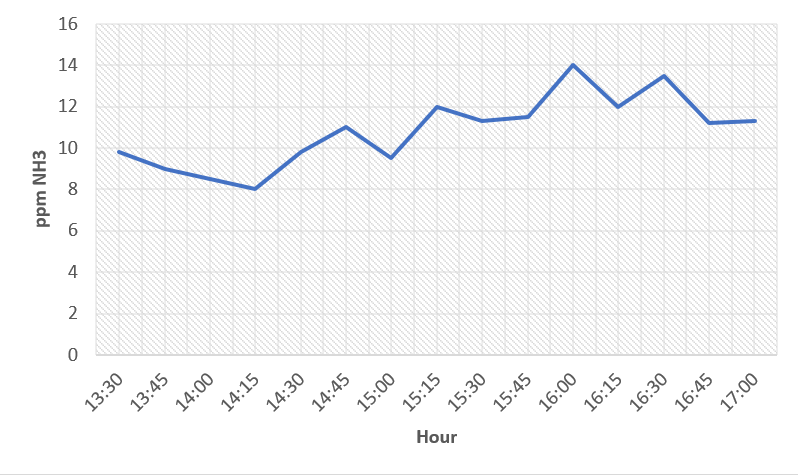
\includegraphics[width=\columnwidth]{mockup grafiek}
    \caption{Voorbeeld grafiek}
\end{figure}








\printbibliography[heading=bibintoc]

\end{document}